\section{Auswertung} 

\subsection{Zählrohrcharakteristik}

\begin{flushleft}
    Die Zählrate N und der Strom $\text{I}_{\text{A}}$ werden in Abhängigkeit von der Betriebsspannung U aufgenommen. 
    Aufgenommen werden Messwerte von $320\,\unit{\volt}$ bis $700\,\unit{\volt}$ in $10\,\unit{\volt}$ Schritten mit einer Messzeit von $t = 60\,\unit{\second}$.
    Die Messwerte befinden sich in der Tabelle \ref{Tabelle1}.
    Das Plateau wird im Bereich von $390\,\unit{\volt}$ bis $620\,\unit{\volt}$ angenommen, mit einer Plateaulänge von $230\,\unit{\volt}$.
\end{flushleft}

\begin{table}[H]
    \centering
    \caption{Die Messwerte der Charakteristik} 
    \label{Tabelle1}
    \begin{tabular} {c  c  c  c}
        \toprule
        {$ \text{U} \mathbin{/} \unit{\volt}$} &
        {$ \text{N} $} &
        {$ \text{N}/ 60\,\unit{\second} \mathbin{/} \frac{1}{\unit{\second}} $} &
        {$ \text{I} \mathbin{/} 10^{-6}\,\unit{\ampere} $} \\
        \midrule
        320 & $ 4643 \pm 68 $ & $ 77,38 \pm 8,79 $ & $ 0,10 \pm 0,05 $  \\
        330 & $ 4772 \pm 69 $ & $ 79,53 \pm 8,91 $ & $ 0,10 \pm 0,05 $  \\
        340 & $ 4898 \pm 69 $ & $ 81,63 \pm 9,03 $ & $ 0,10 \pm 0,05 $  \\
        350 & $ 4976 \pm 70 $ & $ 82,93 \pm 9,10 $ & $ 0,15 \pm 0,05 $  \\
        360 & $ 5070 \pm 71 $ & $ 84,50 \pm 9,19 $ & $ 0,15 \pm 0,05 $  \\
        370 & $ 4975 \pm 70 $ & $ 82,91 \pm 9,10 $ & $ 0,20 \pm 0,05 $  \\
        380 & $ 4839 \pm 69 $ & $ 80,50 \pm 8,98 $ & $ 0,20 \pm 0,05 $  \\
        390 & $ 5062 \pm 71 $ & $ 84,36 \pm 9,18 $ & $ 0,20 \pm 0,05 $  \\
        400 & $ 5110 \pm 71 $ & $ 85,16 \pm 9,22 $ & $ 0,20 \pm 0,05 $  \\
        410 & $ 5105 \pm 71 $ & $ 85,04 \pm 9,22 $ & $ 0,20 \pm 0,05 $  \\
        420 & $ 4827 \pm 69 $ & $ 80,45 \pm 8,96 $ & $ 0,20 \pm 0,05 $  \\
        430 & $ 4943 \pm 70 $ & $ 82,83 \pm 9,07 $ & $ 0,20 \pm 0,05 $  \\
        440 & $ 5098 \pm 71 $ & $ 84,96 \pm 9,21 $ & $ 0,30 \pm 0,05 $  \\
        450 & $ 5049 \pm 71 $ & $ 84,15 \pm 9,17 $ & $ 0,30 \pm 0,05 $  \\
        460 & $ 5116 \pm 71 $ & $ 85,26 \pm 9,23 $ & $ 0,30 \pm 0,05 $  \\
        470 & $ 5096 \pm 71 $ & $ 84,93 \pm 9,21 $ & $ 0,30 \pm 0,05 $  \\
        480 & $ 5020 \pm 70 $ & $ 83,66 \pm 9,14 $ & $ 0,30 \pm 0,05 $  \\
        490 & $ 5011 \pm 70 $ & $ 83,51 \pm 9,13 $ & $ 0,35 \pm 0,05 $  \\
        500 & $ 4995 \pm 70 $ & $ 83,25 \pm 9,12 $ & $ 0,35 \pm 0,05 $  \\
        510 & $ 5092 \pm 71 $ & $ 84,86 \pm 9,21 $ & $ 0,35 \pm 0,05 $  \\
        520 & $ 5181 \pm 71 $ & $ 86,35 \pm 9,29 $ & $ 0,40 \pm 0,05 $  \\
        530 & $ 4998 \pm 70 $ & $ 83,30 \pm 9,12 $ & $ 0,40 \pm 0,05 $  \\
        540 & $ 5180 \pm 71 $ & $ 86,33 \pm 9,29 $ & $ 0,40 \pm 0,05 $  \\
        550 & $ 5147 \pm 71 $ & $ 85,78 \pm 9,26 $ & $ 0,40 \pm 0,05 $  \\
        560 & $ 5086 \pm 71 $ & $ 84,76 \pm 9,20 $ & $ 0,40 \pm 0,05 $  \\
        570 & $ 5171 \pm 71 $ & $ 86,18 \pm 9,28 $ & $ 0,40 \pm 0,05 $  \\
        580 & $ 5155 \pm 71 $ & $ 85,91 \pm 9,26 $ & $ 0,40 \pm 0,05 $  \\
        590 & $ 5005 \pm 70 $ & $ 83,41 \pm 9,13 $ & $ 0,40 \pm 0,05 $  \\
        600 & $ 5193 \pm 72 $ & $ 86,55 \pm 9,30 $ & $ 0,40 \pm 0,05 $  \\
        610 & $ 5119 \pm 71 $ & $ 85,31 \pm 9,23 $ & $ 0,40 \pm 0,05 $  \\
        620 & $ 5097 \pm 71 $ & $ 84,95 \pm 9,21 $ & $ 0,50 \pm 0,05 $  \\
        630 & $ 5222 \pm 72 $ & $ 87,03 \pm 9,32 $ & $ 0,50 \pm 0,05 $  \\
        640 & $ 5245 \pm 72 $ & $ 87,41 \pm 9,34 $ & $ 0,50 \pm 0,05 $  \\
        650 & $ 5206 \pm 72 $ & $ 86,76 \pm 9,31 $ & $ 0,50 \pm 0,05 $  \\
        660 & $ 5216 \pm 72 $ & $ 86,93 \pm 9,32 $ & $ 0,50 \pm 0,05 $  \\
        670 & $ 5263 \pm 72 $ & $ 87,71 \pm 9,34 $ & $ 0,50 \pm 0,05 $  \\
        680 & $ 5303 \pm 72 $ & $ 88,38 \pm 9,40 $ & $ 0,60 \pm 0,05 $  \\
        690 & $ 5390 \pm 73 $ & $ 89,83 \pm 9,47 $ & $ 0,60 \pm 0,05 $  \\
        700 & $ 5302 \pm 72 $ & $ 88,36 \pm 9,40 $ & $ 0,60 \pm 0,05 $  \\
        \bottomrule
    \end{tabular} 
\end{table}

\begin{align*}
    \intertext{Geführt wird eine lineare Regression am Plateau, in der Abbildung \ref{Abbildung6}, mit der Ausgleichsrechnung}
    \text{y} = \text{mx} + \text{b}\,.
\end{align*}

\begin{figure}[H]
    \centering
    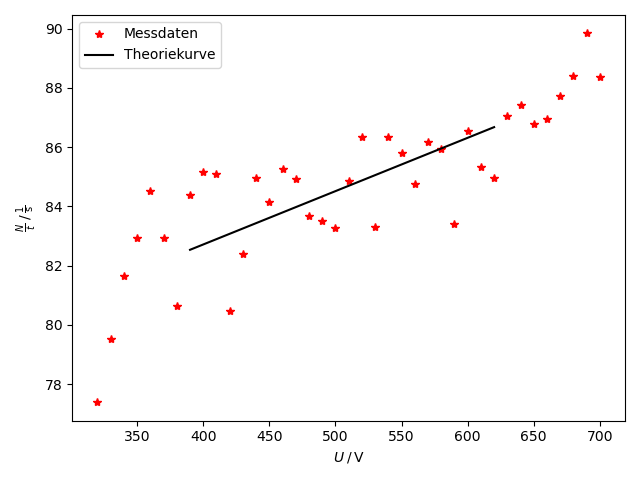
\includegraphics[height=80mm]{bilder/1.png}
    \caption{Die Steigung am Plateau mit der Spannung auf der x-Achse und der Zahlrate geteilt durch $60\,\unit{\second}$ auf der y-Achse. \label{Abbildung6} }
\end{figure}

\begin{align}  
    \intertext{Die Regression liefert die Parameter}
    \text{Steigung m} = ( 0,0084 \pm 0,0039 )\,\frac{1}{\unit{\volt}}\,, \notag \\
    \text{b} = (80,38 \pm 1,99)\,\frac{1}{\unit{\second}} \,, \notag\\
    \to \text{y} = ( 0,0084 \pm 0,0039 )\,\text{x} + (80,38 \pm 1,99)\,.\notag
    \intertext{Aus den Parametern berechnet sich die prozentuale Steigung der Gerade nach der Formel}
    \frac{\text{y}(\text{U}_{2}) - \text{y}(\text{U}_{1})}{\text{y}(\text{U}_{2})} \cdot 100 = 0,69\%.
    \intertext{Demnach beträgt die prozentuale Steigung $ \text{m}_{\%} = 0,69\%$.
    Wird die Steigung durch den Faktor der Plateaulänge dividiert, so folgt für die Steigung}
    \text{m} = 0,978\%\,\,\,\,\, \text{pro}\,\,\,100\,\unit{\volt}\,. \notag
\end{align}

\subsection{Totzeiten}

\begin{align*}
    \intertext{Die Totzeit wird durch das Ablesen am Oszillographen bestimmt.
    Demnach folgt für die abgelesene Totzeit, anhand der Abbildung \ref{Abbildung7}, einen Wert von }
    \text{T}_{\text{Osz.}} = (80 \pm 5)\,\unit{\micro\second}\,.
\end{align*}

\begin{figure}[H]
    \centering
    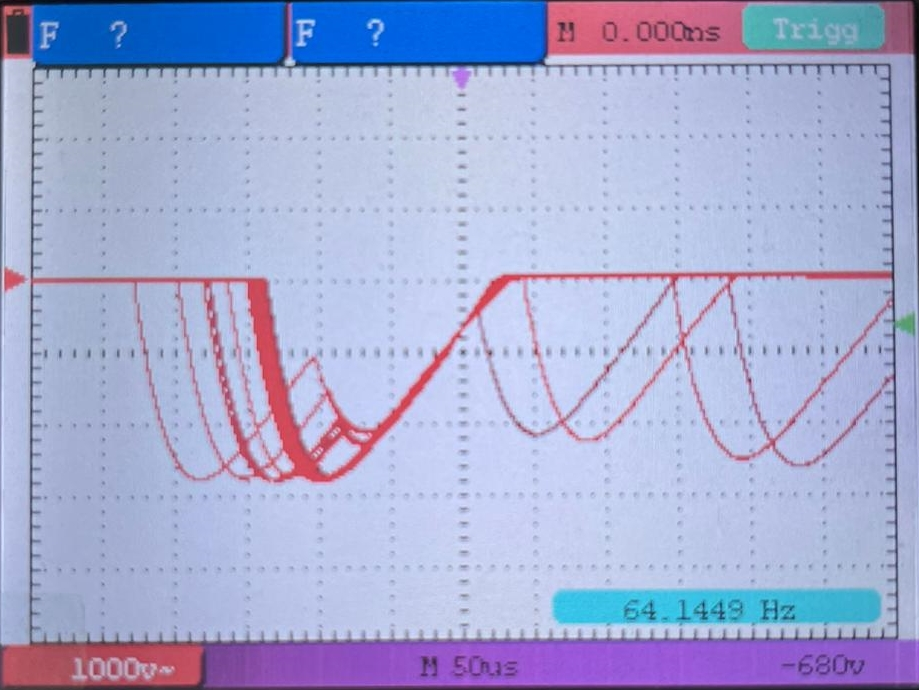
\includegraphics[height=80mm]{bilder/2.jpeg}
    \caption{Tot und Erholungszeit am Oszillographen.\label{Abbildung7} }
\end{figure}

\begin{flushleft}
    Anhand der 2-Quellen-Methode wird erneut die Totzeit bestimmt.
    Ausgenutzt wird bei dieser Methode, dass aufgrund der Totzeit die registrierte Impulszahl $\text{N}_{\text{r}}$ kleiner ist als die wahre Anzahl $\text{N}_{\text{W}}$ der in das Zählrohr gelangten ionisierenden Teilchen.
    Angelegt ist eine Spannung von $500\,\unit{\volt}$ und gemessen wird für $120\,\unit{\second}$.
    Durch die Formel (\ref{2}) berechnet sich die Totzeit.
    Mit den gemessenenWerten aus Tabelle \ref{Tabelle2} ergibt sich
\end{flushleft}

\begin{equation}
    \text{T} = ( 72,29 \pm 4,41 )\cdot 10^{-6} \,\unit{\second}\,. \notag
\end{equation}

\begin{table}[H]
    \centering
    \caption{Messwerte der Totzeiten.} 
    \label{Tabelle2}
    \begin{tabular} {c  c  c}
        \toprule
        {$ \text{N}_{1} $} &
        {$ \text{N}_{2} $} &
        {$ \text{N}_{1+2}$} \\
        \midrule
        $87390 \pm 295$ & $11734 \pm 342$ & $180013 \pm 424$ \\
        \bottomrule
    \end{tabular} 
\end{table}


\subsection{Ladungsmenge pro Teilchen}

\begin{align*}
    \intertext{Mit Hilfe der gemessenen Zählrate und dazugehörigen Ströme, wird nach der Formel (\ref{3}) die Ladungsmengen pro vom Zählrohr freigesetztem Teilchen ermittelt.
    Die Anzahl der Ladungsmenge wird berechnet indem die Ladungsmengen durch die Elementarladung geteilt wird.
    Benutzt werden nur ausgewählte Messwerte, zu sehen in Tabelle \ref{3}. 
    Anschließend wird die Ladungsmenge gegen die Spannung in Abbildung \ref{Abbildung8} aufgetragen und eine lineare Regression mit der Ausgleichsfunktion
    }
    \text{y} = \text{ax} + \text{b}
    \intertext{durchgeführt.}
\end{align*}

\begin{table}[H]
    \centering
    \caption{Messwerte zur Ladungswerk.} 
    \label{Tabelle3}
    \begin{tabular} {c  c  c  c  c  c}
        \toprule
        {$ \text{U} \mathbin{/} \unit{\volt}$} &
        {$ \text{N} $} &
        {$ \text{N}/ 60\,\unit{\second} \mathbin{/} \frac{1}{\unit{\second}} $} &
        {$ \text{I} \mathbin{/} 10^{-6}\,\unit{\ampere} $} & 
        {$ \increment \text{Q} \mathbin{/} 10^{-9}\,\unit{\coulomb} $} &
        {$ \frac{\increment \text{Q}}{\varepsilon_{0}} \mathbin{/} 10^{10} $} \\
        \midrule
        350 & $ 4976 \pm 70 $ & $ 82,93 \pm 9,10 $ & $ 0,15 \pm 0,05 $ & $ 1,80 \pm 0,01 $ & 1,12 \\
        380 & $ 4839 \pm 69 $ & $ 80,50 \pm 8,98 $ & $ 0,20 \pm 0,05 $ & $ 2,47 \pm 0,02 $ & 1,54 \\
        410 & $ 5105 \pm 71 $ & $ 85,04 \pm 9,22 $ & $ 0,20 \pm 0,05 $ & $ 2,35 \pm 0,02 $ & 1,46 \\
        450 & $ 5049 \pm 71 $ & $ 84,15 \pm 9,17 $ & $ 0,30 \pm 0,05 $ & $ 3,56 \pm 0,02 $ & 2,22 \\
        500 & $ 4995 \pm 70 $ & $ 83,25 \pm 9,12 $ & $ 0,35 \pm 0,05 $ & $ 4,20 \pm 0,02 $ & 2,62 \\
        550 & $ 5147 \pm 71 $ & $ 85,78 \pm 9,26 $ & $ 0,40 \pm 0,05 $ & $ 4,66 \pm 0,02 $ & 2,91 \\
        600 & $ 5193 \pm 72 $ & $ 86,55 \pm 9,30 $ & $ 0,40 \pm 0,05 $ & $ 4,62 \pm 0,03 $ & 2,88 \\
        630 & $ 5222 \pm 72 $ & $ 87,03 \pm 9,32 $ & $ 0,50 \pm 0,05 $ & $ 5,74 \pm 0,04 $ & 3,58 \\
        680 & $ 5303 \pm 72 $ & $ 88,38 \pm 9,40 $ & $ 0,60 \pm 0,05 $ & $ 6,78 \pm 0,02 $ & 4,23 \\
        \bottomrule
    \end{tabular} 
\end{table}

\begin{figure}[H]
    \centering
    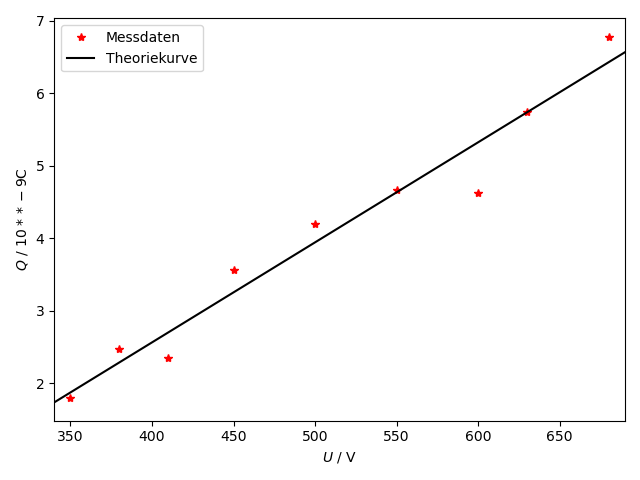
\includegraphics[height=80mm]{bilder/2.png}
    \caption{Die Ladungsmenge gegen die Spannung geplottet, mit der dazugehörigen Ausgleichsgerade. \label{Abbildung8} }
\end{figure}

\begin{align*}
    \intertext{Die Parameter ergeben}
    \text{a} = ( 1,38 \pm 0,11 ) \cdot 10^{-21}\,\frac{\increment \unit{\coulomb}}{\increment \unit{\volt}}\,, \\
    \text{b} = ( -2,95 \pm 0,57 ) \cdot 10^{-19}\, \unit{\coulomb}\,.
\end{align*}